\section{Limitation of Checkpointing to Sequences} \label{sec:5-qual-eval-seq-only}
In this thesis, I have worked exclusively on checkpointing \textit{sequential} neural networks; but what about more general graphs?
The difficulties of handling these with checkpoinitng is possibly its biggest limitation.
In this section, I will show how this limitation arises and evaluate the attempts to tackle it.
I will evaluate the role of my contributions with respect to this work and suggest future work to combine their advantages.

In Section \ref{sec:2-bg-beyond-ff}, I introduced some of the non-linearities that are prevalent today.
For example, consider a ResNet-like architecture \cite{He2016-resnet}, made from a sequence of residual units, which contain skip connections, shown in Figure \ref{fig:5-resnet-arch}.

\begin{figure}[h]
    \centering
    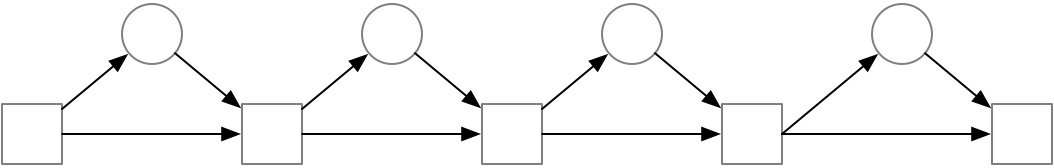
\includegraphics[width=0.6\linewidth]{resnet-checkpointing-demo.png}
    \caption{The ResNet architecture at a high-level, showing the skip connections. Taken from \cite{Bulatov-checkpointing-article}.}
    \label{fig:5-resnet-arch}
\end{figure}

This is almost a sequence.
Can we apply checkpointing to this?
Consider we checkpoint a square node.
Every node to the right of it can indeed be recomputed just from that checkpoint.
In effect, it encapsulates all prior computation.
However, consider checkpointing one of the circular nodes and dropping everything to the left.
The nodes to the right could not be recomputed just from the circular node, as they also require the square node to the left of it;
the circular nodes do not encapsulate all prior computation.

To formalise this notion, what we need is a node that is a \textit{graph separator}.
Every node on the right of this separator will not depend on any of the nodes on the left, only the separator.
That is, the node separates the graph into two \textit{disjoint} subgraphs.

Consider the split-merge architecture shown in Figre \ref{fig:5-split-merge-arch}, such as in GoogleLeNet \cite{Szegedy2015-inception}.

\begin{figure}[h]
    \centering
    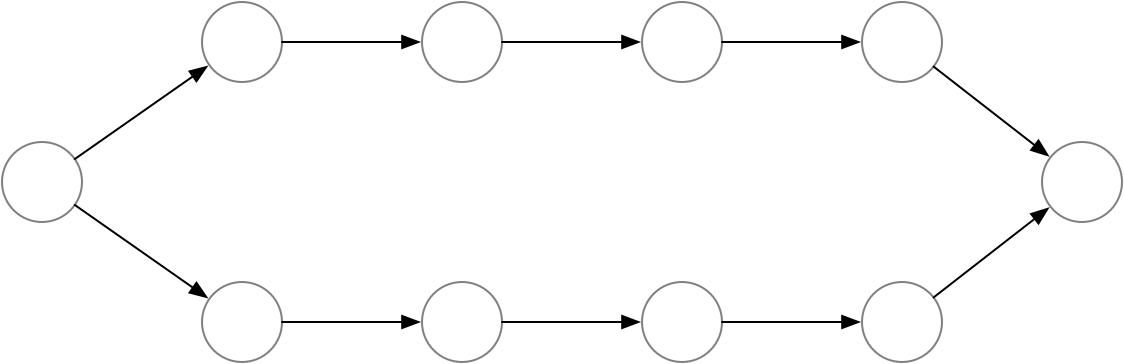
\includegraphics[width=0.6\linewidth]{split-merge-checkpointing-demo.png}
    \caption{A split-merge architecture. Taken from \cite{Bulatov-checkpointing-article}.}
    \label{fig:5-split-merge-arch}
\end{figure}

Again, not all nodes are viable checkpoints; only the `split' and `merge' nodes.
The nodes of the parallel branches cannot be checkpointed invidually.
However, they can be checkpointed \textit{together}.
That is, if we take one node from each branch, this forms a \textit{separating set}, or \textit{bag}, which does split the graph into two disjoint subgraphs.
Equivalently, we have merged nodes into bags such that the network at the bag-level is a sequence.
This is shown in Figure \ref{fig:5-split-merge-separating-set}

\begin{figure}[h]
    \centering
    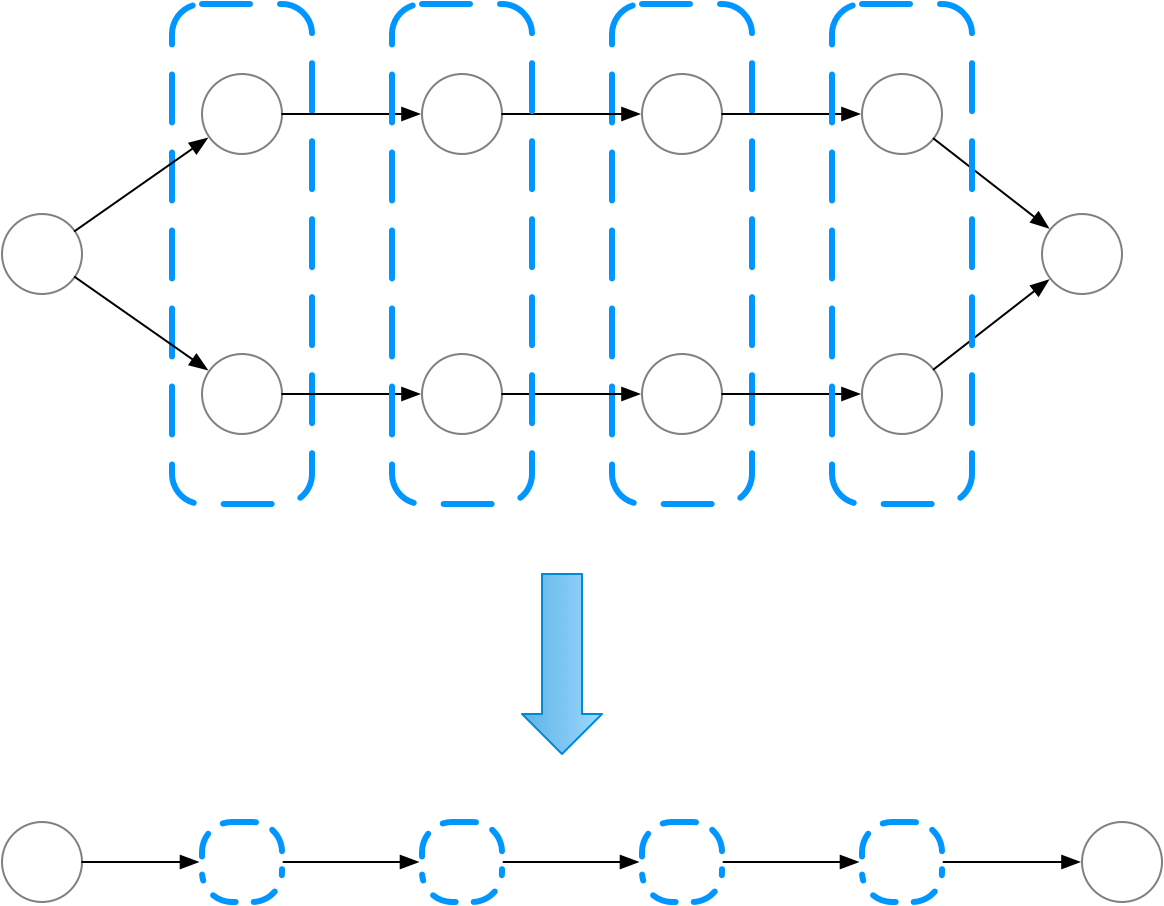
\includegraphics[width=0.6\linewidth]{split-merge-separating-set-checkpointing-demo.png}
    \caption{Separating sets of a split-merge architecture. The dashed lines indicated the merging of nodes into a bag. Taken from \cite{Bulatov-checkpointing-article}.}
    \label{fig:5-split-merge-separating-set}
\end{figure}

More generally, we can checkpoint any node of a computation \textit{tree}, because any node of the tree is a graph separator - it `subsumes' all the computation of its subtrees.
This is shown in Figure \ref{fig:5-tree-checkpointing}.

\begin{figure}[h]
    \centering
    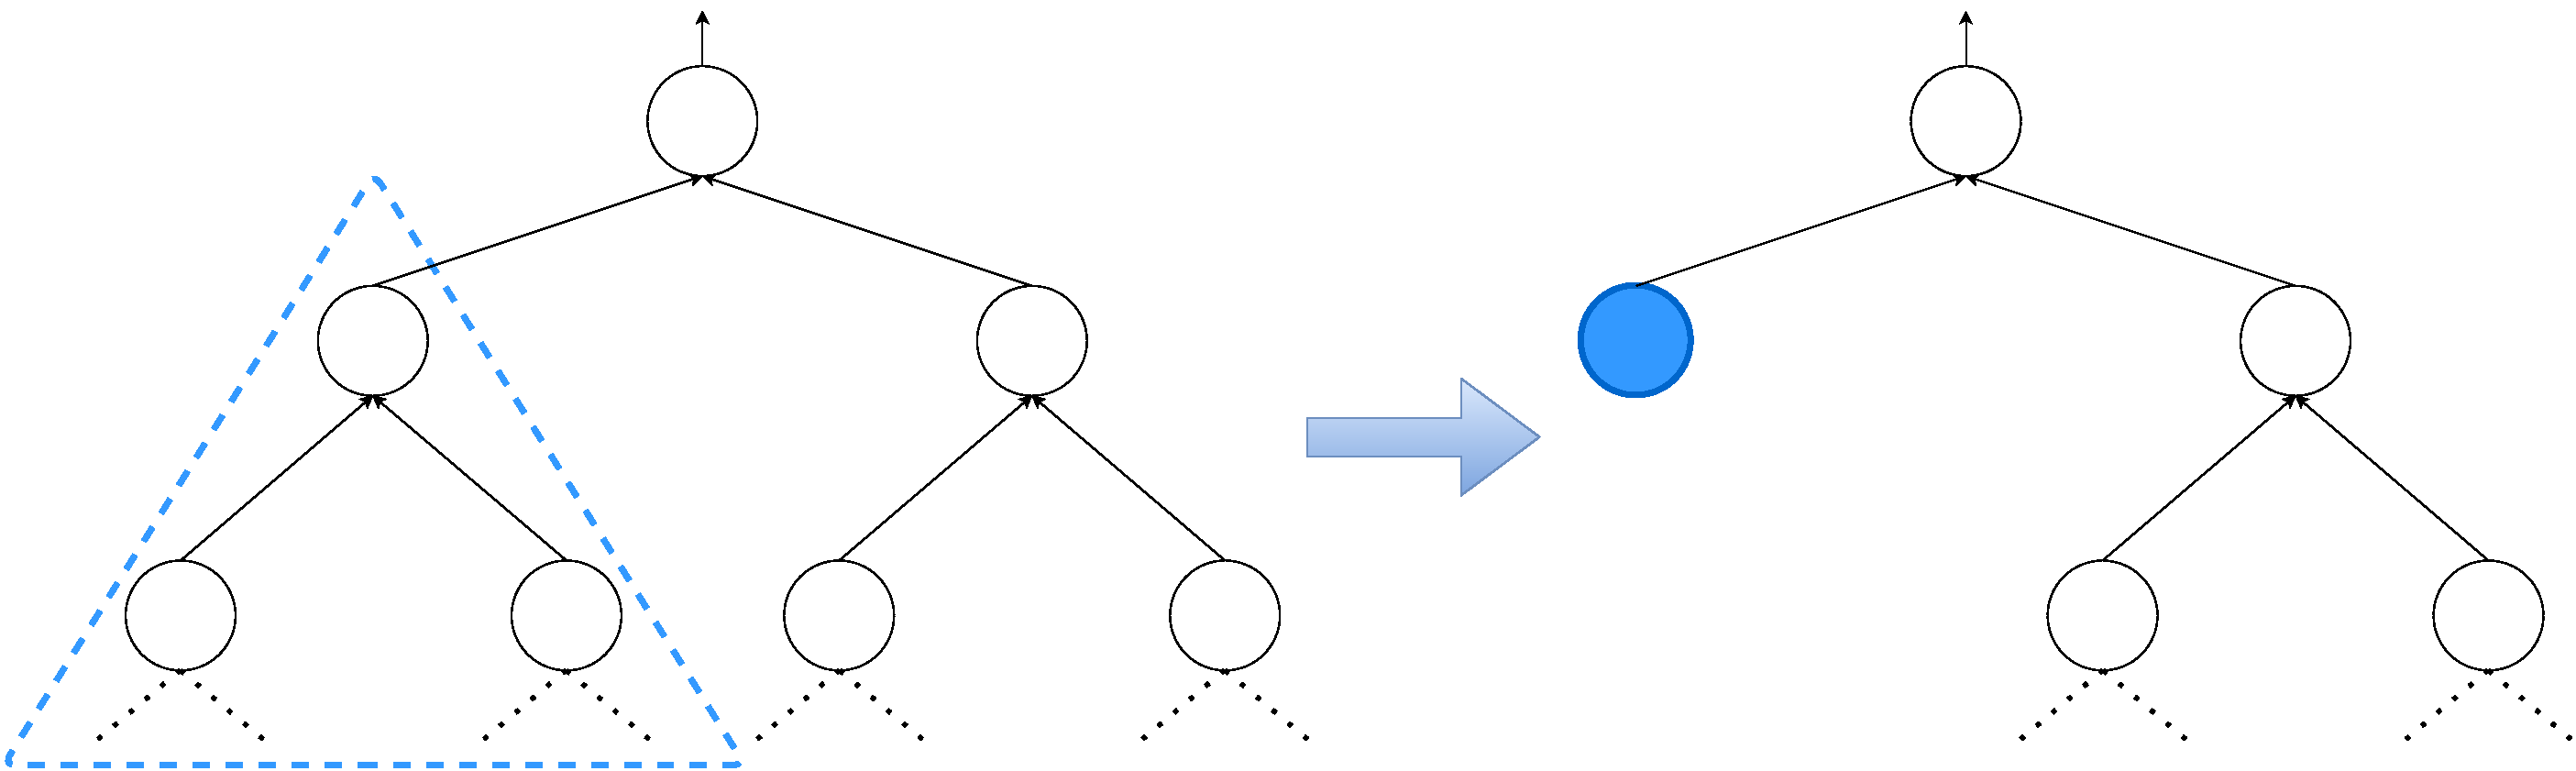
\includegraphics[width=0.78\linewidth]{tree-checkpointing-demo.pdf}
    \caption{Checkpointing on a tree. The blue node on the right `subsumes' all the computation within the dashed lines on the left.}
    \label{fig:5-tree-checkpointing}
\end{figure}

Before we can apply checkpointing to trees, we must solve how to merge nodes of our neural network graphs to form a tree of bags that can be checkpointed at the bag-level.
We need to do this such that we minimise \textit{treewidth} - the maximum number of nodes merged into one bag - in order to be able to perform checkpointing as granularly as possible.
Ideally, we also want to do this without user annotation.

This is known as a \textit{tree decomposition}.
Bodlaender discovered an algorithm that can find the optimal tree decomposition in \(k\)-polynomial time, where \(k\) bounds the treewidth of the graph and is given by the user \cite{Bodlaender2005}.
Looking at the above examples of skip connections and split-merges, we can see that this \(k\) is small, so the algorithm is efficient.
Specifically, for skip connections, the treewidth is three; and for the split-merges it is two.
However, given an abitrary network, we cannot just know this - either the user must tell us or we must compute it ourselves, for which no exact polynomial time algorithms exist.

Say that we have found a tree decomposition for the network, we still need to generalise checkpointing to trees.
First, it would be useful to perform liveness analysis on the tree, as we did in Section \ref{sec:2-4-memory-analysis}, which allowed us to free tensors as we proceeded backwards.
Liu shows how to generalise Sethi's pebble game to trees \cite{Liu1987}.
However, once again each node has a uniform cost.

In 2018, Siskind and Pearlmutter \cite{Siskind2018} generalised Griewank and Walther's \texttt{REVOLVE} checkpointing algorithm to trees, using `divide-and-conquer' checkpointing.
However, as far as I can tell, this also does not take into account precise costs.
Furthermore, like \texttt{REVOLVE} iteself, it is optimal in the sense that it will find the best logarithmic space strategy using multiple recomputations; it will not find the fastest strategy that satisfies a memory budget. 

In 2019, there has been some promising work in the Machine Learning community that generalises checkpointing to arbitrary graphs.
I have only become aware of this work very recently so did not have time to reformulate my solution to build on top of theirs.

The approach of Feng and Huang \cite{Feng2019} can find a checkpointing strategy given an arbitrary graph, without user annotation.
They can even handle arbitrary memory costs.
However, their algorithm minimises the peak memory cost using one recomputation at most; rather than minimising the compute cost given a memory bound with any number of allowed recopmutations.

Kusumoto, Inoue et al. \cite{Kusumoto2019} also generalise checkpointing to arbtirary graphs.
They do indeed minimise computational cost given a memory budget.
However, all is not perfect.
Firstly, like Feng and Huang's approach, they only consider at most one recomputation.
Furthermore, the per-layer costs are not truly precise, profiled costs.
For example, they assume backward tensors are always twice as large as the forwards, something I found not to be the case in my experiments (sometimes they were even ten times as large).
They also model compute costs by saying that convolutional layers are ten times more expensive than all the other layers.
Lastly, they report that their exact dynamic programming solution is too inefficient for large networks; but they also give an approximate solution that gives very near-optimal results.

Nonetheless, both of the above papers represent huge progress, as they generalise to arbitrary graphs.
However, it is clear that a perfect solution is yet to exist;
none of our approaches tick all the boxes.
In the future, we need to find a way to combine the merits of the many approaches.
In particular for me, I would like to look into combining the latter approach, that uses dynamic programming on arbtirary graphs to minimise compute given a memory bound, with mine, that does the same for sequences only, but allows multiple recomputations and takes into account the exact per-operator costs.
